\documentclass[11pt]{article}
\usepackage{amsmath}
\usepackage{amssymb}
\usepackage{graphicx}
\usepackage{tabularx}
\usepackage{fancyhdr}
\usepackage{lastpage}

% Page layout
\usepackage[top=1in, bottom=1in, left=1in, right=1in]{geometry}

% Header and footer
\pagestyle{fancy}
\fancyhf{}
\rfoot{Page \thepage}
\renewcommand{\headrulewidth}{0pt}

% Modified Question command with left-aligned number
\newcommand{\questiona}[2]{
    \noindent\textbf{Q#2.} #1 \hfill \textbf{[1 Mark]}
}

\newcommand{\questionb}[2]{
    \noindent\textbf{Q#2.} #1 \hfill \textbf{[2 Marks]}
}

\begin{document}

% Title section with horizontal line
\begin{center}
    \Large\textbf{GATE 2018 - Mechanical Engineering (ME)} \\
    \large\textbf{General Aptitude and Technical Questions} \\
    \rule{\textwidth}{0.5pt} % Horizontal line below heading
\end{center}

\vspace{0.5cm}

% General Aptitude Section
\section*{General Aptitude}

\questiona{“Going by the \_\_\_\_\_ that many hands make light work, the school \_\_\_\_\_ involved all the students in the task.”}{1}
\begin{enumerate}
    \item[(A)] principle, principal
    \item[(B)] principal, principle
    \item[(C)] principle, principle
    \item[(D)] principal, principal
\end{enumerate}
\vspace{0.5cm}

\questiona{“Her \_\_\_\_\_ should not be confused with miserliness; she is ever willing to assist those in need.”}{2}
\begin{enumerate}
    \item[(A)] cleanliness
    \item[(B)] punctuality
    \item[(C)] frugality
    \item[(D)] greatness
\end{enumerate}
\vspace{0.5cm}

\questiona{Seven machines take 7 minutes to make 7 identical toys. At the same rate, how many minutes would it take for 100 machines to make 100 toys?}{3}
\begin{enumerate}
    \item[(A)] 1
    \item[(B)] 7
    \item[(C)] 100
    \item[(D)] 700
\end{enumerate}
\vspace{0.5cm}

\questiona{A rectangle becomes a square when its length and breadth are reduced by 10 m and 5 m, respectively. During this process, the rectangle loses 650 m\(^2\) of area. What is the area of the original rectangle in square meters?}{4}
\begin{enumerate}
    \item[(A)] 1125
    \item[(B)] 2250
    \item[(C)] 2924
    \item[(D)] 4500
\end{enumerate}
\vspace{0.5cm}

\questiona{A number consists of two digits. The sum of the digits is 9. If 45 is subtracted from the number, its digits are interchanged. What is the number?}{5}
\begin{enumerate}
    \item[(A)] 63
    \item[(B)] 72
    \item[(C)] 81
    \item[(D)] 90
\end{enumerate}
\vspace{0.5cm}

\questionb{For integers \( a, b \) and \( c \), what would be the minimum and maximum values respectively of \( a + b + c \) if \( \log |a| + \log |b| + \log |c| = 0 \)?}{6}
\begin{enumerate}
    \item[(A)] -3 and 3
    \item[(B)] -1 and 1
    \item[(C)] -1 and 3
    \item[(D)] 1 and 3
\end{enumerate}
\vspace{0.5cm}

\questionb{Given that \( a \) and \( b \) are integers and \( a + a^2 b^3 \) is odd, which one of the following statements is correct?}{7}
\begin{enumerate}
    \item[(A)] \( a \) and \( b \) are both odd
    \item[(B)] \( a \) and \( b \) are both even
    \item[(C)] \( a \) is even and \( b \) is odd
    \item[(D)] \( a \) is odd and \( b \) is even
\end{enumerate}
\vspace{0.5cm}

\questionb{From the time the front of a train enters a platform, it takes 25 seconds for the back of the train to leave the platform, while travelling at a constant speed of 54 km/h. At the same speed, it takes 14 seconds to pass a man running at 9 km/h in the same direction as the train. What is the length of the train and that of the platform in meters, respectively?}{8}
\begin{enumerate}
    \item[(A)] 210 and 140
    \item[(B)] 162.5 and 187.5
    \item[(C)] 245 and 130
    \item[(D)] 175 and 200
\end{enumerate}
\vspace{0.5cm}

\questionb{Which of the following functions describe the graph shown in the below figure?}{9}
\begin{center}
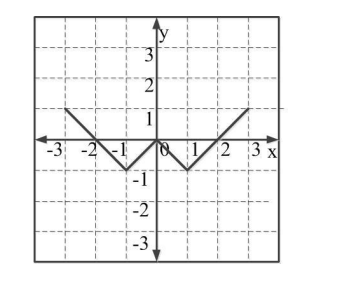
\includegraphics[width=0.5\textwidth]{figures/9.png}
\end{center}
\begin{enumerate}
    \item[(A)] \( y = ||x| + 1| - 2 \)
    \item[(B)] \( y = ||x| - 1| - 1 \)
    \item[(C)] \( y = ||x| + 1| - 1 \)
    \item[(D)] \( y = ||x - 1| - 1| \)
\end{enumerate}
\vspace{0.5cm}

\questionb{Consider the following three statements: \\
(i) Some roses are red. \\
(ii) All red flowers fade quickly. \\
(iii) Some roses fade quickly. \\
Which of the following statements can be logically inferred from the above statements?}{10}
\begin{enumerate}
    \item[(A)] If (i) is true and (ii) is false, then (iii) is false.
    \item[(B)] If (i) is true and (ii) is false, then (iii) is true.
    \item[(C)] If (i) and (ii) are true, then (iii) is true.
    \item[(D)] If (i) and (ii) are false, then (iii) is false.
\end{enumerate}
\vspace{0.5cm}

\section*{Technical Section}

\questiona{Four red balls, four green balls and four blue balls are put in a box. Three balls are pulled out of the box at random one after another without replacement. The probability that all the three balls are red is}{1}
\begin{enumerate}
    \item[(A)] \( \frac{1}{72} \)
    \item[(B)] \( \frac{1}{55} \)
    \item[(C)] \( \frac{1}{36} \)
    \item[(D)] \( \frac{1}{27} \)
\end{enumerate}
\vspace{0.5cm}

\questiona{The rank of the matrix 
\[
\begin{bmatrix}
1 & 1 & 4 \\
1 & 1 & 1 \\
1 & 3 & 7
\end{bmatrix}
\]
is}{2}
\begin{enumerate}
    \item[(A)] 1
    \item[(B)] 2
    \item[(C)] 3
    \item[(D)] 4
\end{enumerate}
\vspace{0.5cm}

\questiona{According to the Mean Value Theorem, for a continuous function \( f(x) \) in the interval \([a,b]\), there exists a value \( \xi \) in this interval such that
\[
\int_a^b f(x) \, dx =
\]}{3}
\begin{enumerate}
    \item[(A)] \( f(b)(b - a) \)
    \item[(B)] \( f(\xi)(b - a) \)
    \item[(C)] \( f(a)(b - \xi) \)
    \item[(D)] 0
\end{enumerate}
\vspace{0.5cm}

\questiona{Let \( F(z) \) be a function of the complex variable \( z = x + iy \), given by
\[
F(z) = i z + k \operatorname{Re}(z) + i \operatorname{Im}(z).
\]
For what value of \( k \) will \( F(z) \) satisfy the Cauchy-Riemann equations?}{4}
\begin{enumerate}
    \item[(A)] 0
    \item[(B)] 1
    \item[(C)] -1
    \item[(D)] \( y \)
\end{enumerate}
\vspace{0.5cm}

\questiona{A bar of uniform cross section and weighing 100 N is held horizontally using two massless and inextensible strings \( S_1 \) and \( S_2 \) as shown in the figure.}{5}
\begin{center}
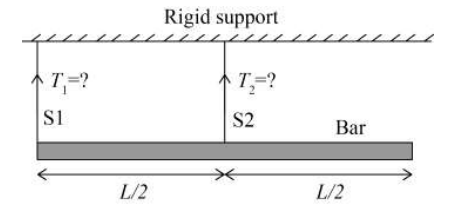
\includegraphics[width=0.5\textwidth]{figures/5.png}
\end{center}
\begin{enumerate}
    \item[(A)] \( T_1 = 100 \text{ N},\ T_2 = 0 \text{ N} \)
    \item[(B)] \( T_1 = 0 \text{ N},\ T_2 = 100 \text{ N} \)
    \item[(C)] \( T_1 = 75 \text{ N},\ T_2 = 25 \text{ N} \)
    \item[(D)] \( T_1 = 25 \text{ N},\ T_2 = 75 \text{ N} \)
\end{enumerate}
\vspace{0.5cm}

\questiona{If \( \sigma_1 \) and \( \sigma_3 \) are the algebraically largest and smallest principal stresses respectively, the value of the maximum shear stress is}{6}
\begin{enumerate}
    \item[(A)] \( \frac{\sigma_1 + \sigma_3}{2} \)
    \item[(B)] \( \frac{\sigma_1 - \sigma_3}{2} \)
    \item[(C)] \( \sqrt{\frac{\sigma_1 + \sigma_3}{2}} \)
    \item[(D)] \( \sqrt{\frac{\sigma_1 - \sigma_3}{2}} \)
\end{enumerate}
\vspace{0.5cm}

\questiona{The equation of motion for a spring-mass system excited by a harmonic force is
\[
M \ddot{x} + Kx = F \cos(\omega t),
\]
where \( M \) is the mass, \( K \) is the spring stiffness, \( F \) is the force amplitude and \( \omega \) is the angular frequency of excitation. Resonance occurs when \( \omega \) is equal to}{7}
\begin{enumerate}
    \item[(A)] \( \frac{M}{K} \)
    \item[(B)] \( \frac{1}{2\pi} \sqrt{\frac{K}{M}} \)
    \item[(C)] \( 2\pi \sqrt{\frac{K}{M}} \)
    \item[(D)] \( \sqrt{\frac{K}{M}} \)
\end{enumerate}
\vspace{0.5cm}

\questiona{For an Oldham coupling used between two shafts, which among the following statements are correct? \\
I. Torsional load is transferred along shaft axis. \\
II. A velocity ratio of 1:2 between shafts is obtained without using gears. \\
III. Bending load is transferred transverse to shaft axis. \\
IV. Rotation is transferred along shaft axis.}{8}
\begin{enumerate}
    \item[(A)] I and III
    \item[(B)] I and IV
    \item[(C)] II and III
    \item[(D)] II and IV
\end{enumerate}
\vspace{0.5cm}

\questiona{For a two-dimensional incompressible flow field given by \( \vec{u} = A (\hat{i} y - \hat{j} x) \), where \( A > 0 \), which one of the following statements is FALSE?}{9}
\begin{enumerate}
    \item[(A)] It satisfies continuity equation.
    \item[(B)] It is unidirectional when \( x \rightarrow 0 \) and \( y \rightarrow \infty \).
    \item[(C)] Its streamlines are given by \( xy = \text{constant} \).
    \item[(D)] It is irrotational.
\end{enumerate}
\vspace{0.5cm}

\questiona{Which one of the following statements is correct for a superheated vapour?}{10}
\begin{enumerate}
    \item[(A)] Its pressure is less than the saturation pressure at a given temperature.
    \item[(B)] Its temperature is less than the saturation temperature at a given pressure.
    \item[(C)] Its volume is less than the volume of the saturated vapour at a given temperature.
    \item[(D)] Its enthalpy is less than the enthalpy of the saturated vapour at a given pressure.
\end{enumerate}
\vspace{0.5cm}

\questiona{In a linearly hardening plastic material, the true stress beyond initial yielding}{11}
\begin{enumerate}
    \item[(A)] increases linearly with the true strain
    \item[(B)] decreases linearly with the true strain
    \item[(C)] first increases linearly and then decreases linearly with the true strain
    \item[(D)] remains constant
\end{enumerate}
\vspace{0.5cm}

\questiona{The type of weld represented by the shaded region in the figure is}{12}
\begin{center}
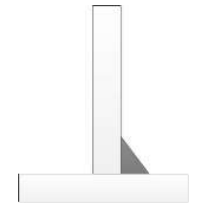
\includegraphics[width=0.5\textwidth]{figures/12.png}
\end{center}
\begin{enumerate}
    \item[(A)] groove
    \item[(B)] spot
    \item[(C)] fillet
    \item[(D)] plug
\end{enumerate}
\vspace{0.5cm}

\questiona{Using the Taylor’s tool life equation with exponent \( n = 0.5 \), if the cutting speed is reduced by 50\%, the ratio of new tool life to original tool life is}{13}
\begin{enumerate}
    \item[(A)] 4
    \item[(B)] 2
    \item[(C)] 1
    \item[(D)] 0.5
\end{enumerate}
\vspace{0.5cm}

\questiona{A grinding ratio of 200 implies that the}{14}
\begin{enumerate}
    \item[(A)] grinding wheel wears 200 times the volume of the material removed
    \item[(B)] grinding wheel wears 0.005 times the volume of the material removed
    \item[(C)] aspect ratio of abrasive particles used in the grinding wheel is 200
    \item[(D)] ratio of volume of abrasive particle to that of grinding wheel is 200
\end{enumerate}
\vspace{0.5cm}

\questiona{Interpolator in a CNC machine}{15}
\begin{enumerate}
    \item[(A)] controls spindle speed
    \item[(B)] coordinates axes movements
    \item[(C)] operates tool changer
    \item[(D)] commands canned cycle
\end{enumerate}
\vspace{0.5cm}

\questiona{The time series forecasting method that gives equal weightage to each of the \( m \) most recent observations is}{16}
\begin{enumerate}
    \item[(A)] Moving average method
    \item[(B)] Exponential smoothing with linear trend
    \item[(C)] Triple Exponential smoothing
    \item[(D)] Kalman Filter
\end{enumerate}
\vspace{0.5cm}

\questiona{The number of atoms per unit cell and the number of slip systems, respectively, for a face-centered cubic (FCC) crystal are}{17}
\begin{enumerate}
    \item[(A)] 3, 3
    \item[(B)] 3, 12
    \item[(C)] 4, 12
    \item[(D)] 4, 48
\end{enumerate}
\vspace{0.5cm}

\questiona{A six-faced fair dice is rolled five times. The probability (in \%) of obtaining “ONE” at least four times is}{18}
\begin{enumerate}
    \item[(A)] 33.3
    \item[(B)] 3.33
    \item[(C)] 0.33
    \item[(D)] 0.0033
\end{enumerate}
\vspace{0.5cm}

\questiona{A steel column of rectangular section (15 mm × 10 mm) and length 1.5 m is simply supported at both ends. Assuming modulus of elasticity, \( E = 200 \) GPa for steel, the critical axial load (in kN) is \_\_\_\_ (correct to two decimal places).}{19}
\vspace{0.5cm}

\questiona{A four bar mechanism is made up of links of length 100, 200, 300 and 350 mm. If the 350 mm link is fixed, the number of links that can rotate fully is \_\_\_\_\_\_\_.}{20}
\vspace{0.5cm}

\questiona{If the wire diameter of a compressive helical spring is increased by 2\%, the change in spring stiffness (in \%) is \_\_\_\_\_\_ (correct to two decimal places).}{21}
\vspace{0.5cm}

\questiona{A flat plate of width \( L = 1 \) m is pushed down with a velocity \( U = 0.01 \) m/s towards a wall resulting in the drainage of the fluid between the plate and the wall as shown in the figure. Assume two-dimensional incompressible flow and that the plate remains parallel to the wall. The average velocity, \( u_{\text{avg}} \), of the fluid (in m/s) draining out at the instant shown in the figure is \_\_\_\_\_\_\_\_ (correct to three decimal places).}{22}
\begin{center}
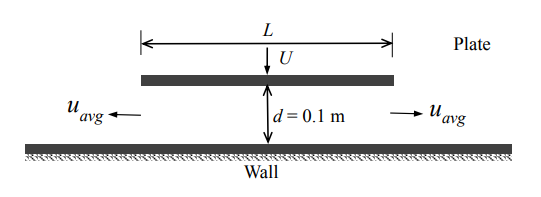
\includegraphics[width=0.7\textwidth]{figures/22.png}
\end{center}
\vspace{0.5cm}

\questiona{An ideal gas undergoes a process from state 1 (\( T_1 = 300 \) K, \( p_1 = 100 \) kPa) to state 2 (\( T_2 = 600 \) K, \( p_2 = 500 \) kPa). The specific heats of the ideal gas are: \( c_p = 1 \) kJ/kg-K and \( c_v = 0.7 \) kJ/kg-K. The change in specific entropy of the ideal gas from state 1 to state 2 (in kJ/kg-K) is \_\_\_\_\_\_ (correct to two decimal places).}{23}
\vspace{0.5cm}

\questiona{For a Pelton wheel with a given water jet velocity, the maximum output power from the Pelton wheel is obtained when the ratio of the bucket speed to the water jet speed is \_\_\_\_ (correct to two decimal places).}{24}
\vspace{0.5cm}

\questiona{The height (in mm) for a 125 mm sine bar to measure a taper of \( 27^\circ 32' \) on a flat work piece is \_\_\_\_ (correct to three decimal places).}{25}
\vspace{0.5cm}

\questionb{Let \( X_1, X_2 \) be two independent normal random variables with means \( \mu_1, \mu_2 \) and standard deviations \( \sigma_1, \sigma_2 \), respectively. Consider \( Y = X_1 - X_2 \); \( \mu_1 = \mu_2 = 1, \sigma_1 = 1, \sigma_2 = 2 \). Then,}{26}
\begin{enumerate}
    \item[(A)] \( Y \) is normally distributed with mean 0 and variance 1
    \item[(B)] \( Y \) is normally distributed with mean 0 and variance 5
    \item[(C)] \( Y \) has mean 0 and variance 5, but is NOT normally distributed
    \item[(D)] \( Y \) has mean 0 and variance 1, but is NOT normally distributed
\end{enumerate}
\vspace{0.5cm}

\questionb{The value of the integral
\[
\iint_S \vec{r} \cdot \vec{n} \, dS
\]
over the closed surface \( S \) bounding a volume \( V \), where \( \vec{r} = x\hat{i} + y\hat{j} + z\hat{k} \) is the position vector and \( \vec{n} \) is the normal to the surface \( S \), is}{27}
\begin{enumerate}
    \item[(A)] \( V \)
    \item[(B)] \( 2V \)
    \item[(C)] \( 3V \)
    \item[(D)] \( 4V \)
\end{enumerate}
\vspace{0.5cm}

\questionb{A point mass is shot vertically up from ground level with a velocity of 4 m/s at time \( t = 0 \). It loses 20\% of its impact velocity after each collision with the ground. Assuming that the acceleration due to gravity is 10 m/s\(^2\) and that air resistance is negligible, the mass stops bouncing and comes to complete rest on the ground after a total time (in seconds) of}{28}
\begin{enumerate}
    \item[(A)] 1
    \item[(B)] 2
    \item[(C)] 4
    \item[(D)] \( \infty \)
\end{enumerate}
\vspace{0.5cm}

\questionb{The state of stress at a point, for a body in plane stress, is shown in the figure below. If the minimum principal stress is 10 kPa, then the normal stress \( \sigma_y \) (in kPa) is}{29}
\begin{center}
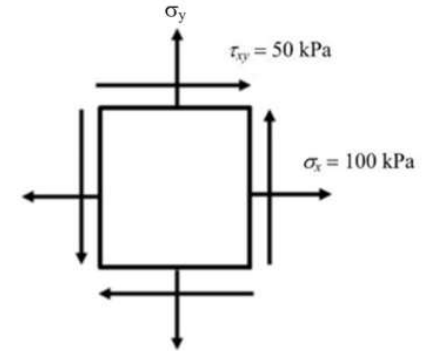
\includegraphics[width=0.5\textwidth]{figures/29.png}
\end{center}
\begin{enumerate}
    \item[(A)] 9.45
    \item[(B)] 18.88
    \item[(C)] 37.78
    \item[(D)] 75.50
\end{enumerate}
\vspace{0.5cm}

\questionb{An epicyclic gear train is shown in the figure below. The number of teeth on the gears A, B and D are 20, 30 and 20, respectively. Gear C has 80 teeth on the inner surface and 100 teeth on the outer surface. If the carrier arm AB is fixed and the sun gear A rotates at 300 rpm in the clockwise direction, then the rpm of D in the clockwise direction is}{30}
\begin{center}
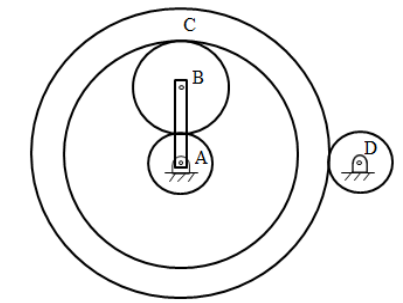
\includegraphics[width=0.5\textwidth]{figures/30.png}
\end{center}
\begin{enumerate}
    \item[(A)] 240
    \item[(B)] -240
    \item[(C)] 375
    \item[(D)] -375
\end{enumerate}
\vspace{0.5cm}

\questionb{A carpenter glues a pair of cylindrical wooden logs by bonding their end faces at an angle of \( \theta = 30^\circ \) as shown in the figure. \\
The glue used at the interface fails if: \\
Criterion 1: the maximum normal stress exceeds 2.5 MPa. \\
Criterion 2: the maximum shear stress exceeds 1.5 MPa. \\
Assume that the interface fails before the logs fail. When a uniform tensile stress of 4 MPa is applied, the interface}{31}
\begin{center}
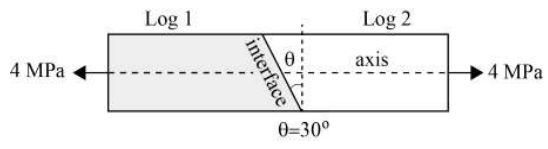
\includegraphics[width=0.5\textwidth]{figures/31.png}
\end{center}
\begin{enumerate}
    \item[(A)] fails only because of criterion 1
    \item[(B)] fails only because of criterion 2
    \item[(C)] fails because of both criteria 1 and 2
    \item[(D)] does not fail
\end{enumerate}
\vspace{0.5cm}

\questionb{A self-aligning ball bearing has a basic dynamic load rating (\( C_{10} \), for \( 10^6 \) revolutions) of 35 kN. If the equivalent radial load on the bearing is 45 kN, the expected life (in \( 10^6 \) revolutions) is}{32}
\begin{enumerate}
    \item[(A)] below 0.5
    \item[(B)] 0.5 to 0.8
    \item[(C)] 0.8 to 1.0
    \item[(D)] above 1.0
\end{enumerate}
\vspace{0.5cm}

\questionb{A tank open at the top with a water level of 1 m, as shown in the figure, has a hole at a height of 0.5 m. A free jet leaves horizontally from the smooth hole. The distance \( X \) (in m) where the jet strikes the floor is}{33}
\begin{center}
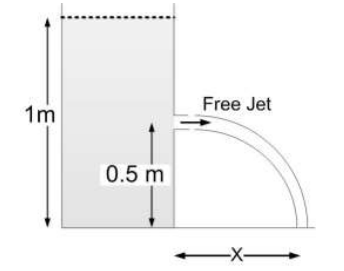
\includegraphics[width=0.5\textwidth]{figures/33.png}
\end{center}
\begin{enumerate}
    \item[(A)] 0.5
    \item[(B)] 1.0
    \item[(C)] 2.0
    \item[(D)] 4.0
\end{enumerate}
\vspace{0.5cm}

\questionb{In a Lagrangian system, the position of a fluid particle in a flow is described as \( x = x_0 e^{-kt} \) and \( y = y_0 e^{kt} \) where \( t \) is the time while \( x_0, y_0 \), and \( k \) are constants. The flow is}{34}
\begin{enumerate}
    \item[(A)] unsteady and one-dimensional
    \item[(B)] steady and two-dimensional
    \item[(C)] steady and one-dimensional
    \item[(D)] unsteady and two-dimensional
\end{enumerate}
\vspace{0.5cm}

\questionb{The maximum reduction in cross-sectional area per pass (\( R \)) of a cold wire drawing process is 
\[
R = 1 - \left( \frac{1}{1 + n} \right)^{n},
\]
where \( n \) represents the strain hardening coefficient. For the case of a perfectly plastic material, \( R \) is}{35}
\begin{enumerate}
    \item[(A)] 0.865
    \item[(B)] 0.826
    \item[(C)] 0.777
    \item[(D)] 0.632
\end{enumerate}
\vspace{0.5cm}

\questionb{The percentage scrap in a sheet metal blanking operation of a continuous strip of sheet metal as shown in the figure is \_\_\_\_\_ (correct to two decimal places).}{36}
\begin{center}
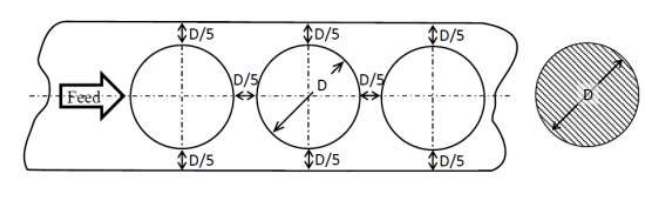
\includegraphics[width=0.7\textwidth]{figures/36.png}
\end{center}
\vspace{0.5cm}

\questionb{An explicit forward Euler method is used to numerically integrate the differential equation \( \frac{dy}{dt} = y \) using a time step of 0.1. With the initial condition \( y(0) = 1 \), the value of \( y(1) \) computed by this method is \_\_\_\_\_ (correct to two decimal places).}{37}
\vspace{0.5cm}

\questionb{Let \( F(s) \) be the Laplace transform of the function \( f(t) = 2t e^{-2t} \). The value of \( F(1) \) is \_\_\_\_\_ (correct to two decimal places).}{38}
\vspace{0.5cm}

\questionb{A simply supported beam of width 100 mm, height 200 mm and length 4 m is carrying a uniformly distributed load of intensity 10 kN/m. The maximum bending stress (in MPa) in the beam is \_\_\_\_\_ (correct to one decimal place).}{39}
\begin{center}
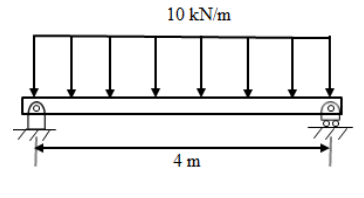
\includegraphics[width=0.5\textwidth]{figures/39.png}
\end{center}
\vspace{0.5cm}

\questionb{A machine of mass \( m = 200 \) kg is supported on two mounts, each of stiffness \( k = 10 \) kN/m. The machine is subjected to an external force \( F(t) = 50 \cos(5t) \) N. Assuming only vertical translatory motion, the magnitude of the dynamic force (in N) transmitted from each mount to the ground is \_\_\_\_\_ (correct to two decimal places).}{40}
\begin{center}
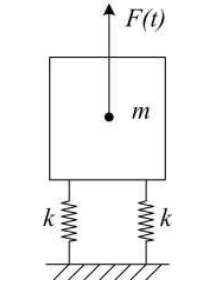
\includegraphics[width=0.4\textwidth]{figures/40.png}
\end{center}
\vspace{0.5cm}

\questionb{A slider crank mechanism is shown in the figure. At some instant, the crank angle is \( 45^\circ \) and a force of 40 N is acting towards the left on the slider. The length of the crank is 30 mm and the connecting rod is 70 mm. Ignoring the effect of gravity, friction and inertial forces, the magnitude of the crankshaft torque (in Nm) needed to keep the mechanism in equilibrium is \_\_\_\_\_ (correct to two decimal places).}{41}
\begin{center}
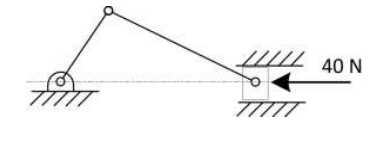
\includegraphics[width=0.5\textwidth]{figures/41.png}
\end{center}
\vspace{0.5cm}

\questionb{A sprinkler shown in the figure rotates about its hinge point in a horizontal plane due to water flow discharged through its two exit nozzles. The total flow rate \( Q \) through the sprinkler is 1 litre/sec and the cross-sectional area of each exit nozzle is 1 cm\(^2\). Assuming equal flow rate through both arms and a frictionless hinge, the steady state angular speed of rotation (in rad/s) of the sprinkler is \_\_\_\_\_ (correct to two decimal places).}{42}
\begin{center}
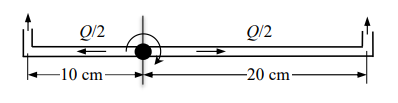
\includegraphics[width=0.5\textwidth]{figures/42.png}
\end{center}
\vspace{0.5cm}

\questionb{A solid block of 2.0 kg mass slides steadily at a velocity \( V \) along a vertical wall as shown in the figure below. A thin oil film of thickness \( h = 0.15 \) mm provides lubrication between the block and the wall. The surface area of the face of the block in contact with the oil film is 0.04 m\(^2\). The velocity distribution within the oil film gap is linear. Take dynamic viscosity of oil as \( 7 \times 10^{-3} \) Pa-s and acceleration due to gravity as 10 m/s\(^2\). Neglect weight of the oil. The terminal velocity \( V \) (in m/s) of the block is \_\_\_\_\_ (correct to one decimal place).}{43}
\begin{center}
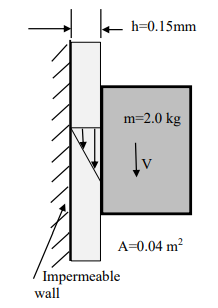
\includegraphics[width=0.5\textwidth]{figures/43.png}
\end{center}
\vspace{0.5cm}

\questionb{A tank of volume 0.05 m\(^3\) contains a mixture of saturated water and saturated steam at 200\(^\circ\)C. The mass of the liquid present is 8 kg. The entropy (in kJ/kg K) of the mixture is \_\_\_\_\_ (correct to two decimal places). \\
Property data for saturated steam and water at 200\(^\circ\)C: \\
\( v_f = 0.001157 \) m\(^3\)/kg, \( v_g = 0.12736 \) m\(^3\)/kg, \( s_f = 2.3309 \) kJ/kg-K, \( s_{fg} = 4.1014 \) kJ/kg-K.}{44}
\vspace{0.5cm}

\questionb{Steam flows through a nozzle at a mass flow rate of \( \dot{m} = 1.0 \) kg/s with a heat loss of 5 kW. The enthalpies at inlet and exit are 2500 kJ/kg and 2350 kJ/kg, respectively. Assuming negligible velocity at inlet (\( C_1 \approx 0 \)), the velocity \( C_2 \) of steam (in m/s) at the nozzle exit is \_\_\_\_\_ (correct to two decimal places).}{45}
\begin{center}
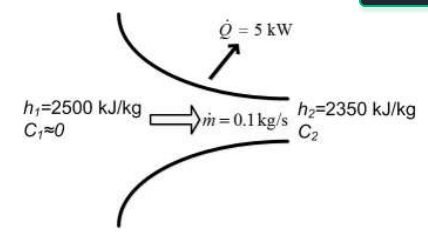
\includegraphics[width=0.5\textwidth]{figures/45.png}
\end{center}
\vspace{0.5cm}

\questionb{An engine working on air standard Otto cycle is supplied with air at 0.1 MPa and 35°C. The compression ratio is 8. The heat supplied is 500 kJ/kg. \\
Property data for air: \( c_p = 1.005 \) kJ/kg·K, \( c_v = 0.718 \) kJ/kg·K, \( R = 0.287 \) kJ/kg·K. \\
The maximum temperature (in K) of the cycle is \_\_\_\_\_ (correct to one decimal place).}{46}
\vspace{0.5cm}

\questionb{A plane slab of thickness \( L \) and thermal conductivity \( k \) is heated with a fluid on one side (P), and the other side (Q) is maintained at a constant temperature, \( T_Q = 25^\circ \)C, as shown in the figure. The fluid is at 45°C and the surface heat transfer coefficient \( h = 10 \) W/m\(^2\)·K. The steady state temperature \( T_P \) (in °C) of the side which is exposed to the fluid is \_\_\_\_\_ (correct to two decimal places).}{47}
\begin{center}
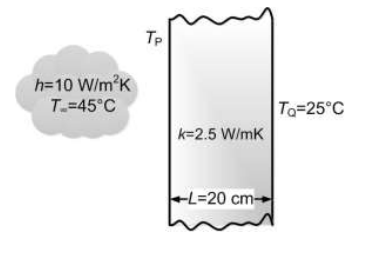
\includegraphics[width=0.5\textwidth]{figures/47.png}
\end{center}
\vspace{0.5cm}

\questionb{The true stress ( \( \sigma \) ) - true strain ( \( \varepsilon \) ) diagram of a strain hardening material is shown in figure. First, there is loading up to point A ( \( \sigma = 500 \) MPa, \( \varepsilon = 0.5 \) ), and then unloading up to point B ( \( \sigma = 100 \) MPa). Given that the Young’s modulus \( E = 200 \) GPa, the natural strain at point B ( \( \varepsilon_B \) ) is \_\_\_\_\_ (correct to three decimal places).}{48}
\begin{center}
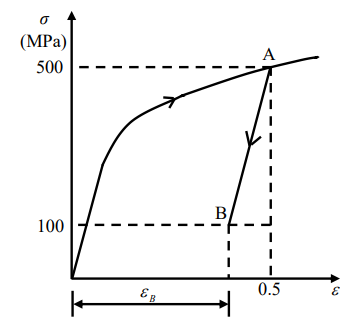
\includegraphics[width=0.5\textwidth]{figures/48.png}
\end{center}
\vspace{0.5cm}

\questionb{An orthogonal cutting operation is being carried out in which uncut thickness is 0.010 mm, cutting speed is 130 m/min, rake angle is \( 15^\circ \), and width of cut is 6 mm. It is observed that the chip thickness is 0.015 mm, the cutting force is 60 N and the thrust force is 25 N. The ratio of friction energy to total energy is \_\_\_\_\_ (correct to two decimal places).}{49}
\vspace{0.5cm}

\questionb{A bar is compressed to half of its original length. The magnitude of true strain produced in the deformed bar is \_\_\_\_\_ (correct to two decimal places).}{50}
\vspace{0.5cm}

\questionb{The minimum value of \( 3x + 5y \) such that: \\
\[
\begin{aligned}
3x + 5y &\leq 15 \\
4x + 9y &\leq 8 \\
13x + 2y &\leq 2 \\
x &\geq 0, \quad y \geq 0
\end{aligned}
\]
is \_\_\_\_\_.}{51}
\vspace{0.5cm}

\questionb{Processing times (including setup times) and due dates for six jobs waiting to be processed at a work centre are given in the table. The average tardiness (in days) using shortest processing time rule is \_\_\_\_\_ (correct to two decimal places).}{52}

\begin{center}
\begin{tabular}{|c|c|c|}
\hline
\textbf{Job} & \textbf{Processing time (days)} & \textbf{Due date (days)} \\
\hline
A & 3 & 8 \\
B & 7 & 16 \\
C & 4 & 4 \\
D & 9 & 18 \\
E & 5 & 17 \\
F & 13 & 19 \\
\hline
\end{tabular}
\end{center}
\vspace{0.5cm}

\questionb{The schematic of an external drum rotating clockwise engaging with a short shoe is shown in the figure. The shoe is mounted at point Y on a rigid lever XYZ hinged at point X. A force \( F = 100 \) N is applied at the free end of the lever as shown. Given that the coefficient of friction between the shoe and the drum is 0.3, the braking torque (in Nm) applied on the drum is \_\_\_\_\_ (correct to two decimal places).}{53}
\begin{center}
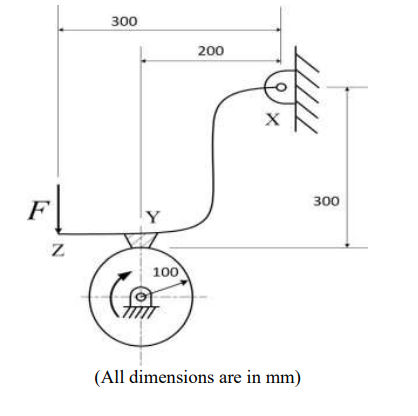
\includegraphics[width=0.5\textwidth]{figures/53.png}
\end{center}
\vspace{0.5cm}

\questionb{Block P of mass 2 kg slides down the surface and has a speed 20 m/s at the lowest point Q, where the local radius of curvature is 2 m as shown in the figure. Assuming \( g = 10 \) m/s\(^2\), the normal force (in N) at Q is \_\_\_\_\_ (correct to two decimal places).}{54}
\begin{center}
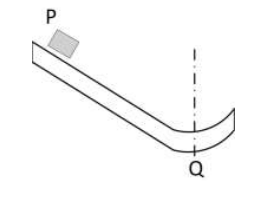
\includegraphics[width=0.5\textwidth]{figures/54.png}
\end{center}
\vspace{0.5cm}

\questionb{An electrochemical machining (ECM) is to be used to cut a through hole into a 12 mm thick aluminum plate. The hole has a rectangular cross-section, 10 mm × 30 mm. The ECM operation will be accomplished in 2 minutes, with efficiency of 90\%. Assuming specific removal rate for aluminum as \( 3.44 \times 10^{-2} \) mm\(^3\)/(A·s), the current (in A) required is \_\_\_\_\_ (correct to two decimal places).}{55}
\vspace{0.5cm}

% End of paper
\vspace{5cm}
\begin{center}
\textbf{END OF THE QUESTION PAPER} \\
\rule{\textwidth}{0.5pt}
\end{center}

\end{document}
